\documentclass[11pt]{article}

%Format and referencing 
\usepackage[letterpaper,top=2cm,bottom=2cm,left=1.5cm,right=2cm,marginparwidth=1.75cm]{geometry} % for setting margins VERY IMPORTANT!
\usepackage{hyperref}  % for referencing equations 
\usepackage{biblatex}  % for referencing articles 
\addbibresource{Bib.bib}


%math packages 
\usepackage{mathtools}  % allows pre-scripts and other neiche math features
\usepackage{amsmath} % equation related commands 
\usepackage{amssymb} % Fancy R ,C and other set fonts using mathbb{}
\usepackage{braket}   % for Dirac notation 
\usepackage{mathrsfs}  % for the mathscr text 
\usepackage{bbm} % for identity matrix

% miscellaneous
\usepackage{empheq}   % for formatting custon math boxs
\usepackage{xcolor}   % allows the defining of colours 
\usepackage[most]{tcolorbox}  % custom math boxs
\usepackage[utf8]{inputenc}   % redundant since 2018? 
%(I'm not taking out in case it breaks stuff)

\usepackage{graphicx}   % alows image insertion 
\usepackage{float}  % for making images o where you want 
\usepackage{parskip} % for getting red of paragraph indent 

\usepackage{comment} %easier multi line comments 
 \usepackage{tabularx} % for formatting tables 
 \usepackage{titling} % for making Title a variable that can be used in header 
 \usepackage{environ} % for creating and modifying environments 
 \usepackage[explicit]{titlesec}
 % for making section titles variables that can be used in header 
\usepackage{fancyhdr} % for fancy headers 

% Random commands and what not 
\numberwithin{equation}{section}

\setlength{\droptitle}{3em} 

{\Huge  
\title{Standard Model}
\author{Thomas Brosnan}
\date{Notes taken in Professor Ruth Britto's class, Hillary term 2025}
}

\DeclarePairedDelimiterXPP\BigOSI[2]%
  {\mathcal{O}}{(}{)}{}%
  {\SI{#1}{#2}}

\newtcbox{\mymath}[1][]{%
    nobeforeafter, math upper, tcbox raise base,
    enhanced, colframe=blue!30!black,
    colback=blue!30, boxrule=1pt,
    #1}
\tcbset{highlight math style={boxsep=2mm,,colback=blue!0!green!0!red!0!}}

\newenvironment{bux}{\empheq[box=\tcbhighmath]{align}}{\endempheq}
\newenvironment{bux*}{\empheq[box=\tcbhighmath]{align*}}{\endempheq}
\renewenvironment{flalign}{\vspace{-3mm}\empheq[box=\tcbhighmath]{align}}{\endempheq}
\renewenvironment{flalign*}{\vspace{-3mm}\empheq[box=\tcbhighmath]{align*}}{\endempheq}
%\renewenvironment{align}{\vspace{-5mm}\begin{align}}{\end{align}}
%\renewenvironment{align*}{\vspace{-5mm}\begin{align*}}{\end{align*}}
\renewenvironment{alignat}{\empheq{align*}}{\endempheq}


\newcommand{\hsp}{\hspace{8pt}}

\newcommand{\I}[1]{\emph{#1}}

\newcommand*{\sectionFont}{%
  \LARGE\bfseries
}

\newenvironment{eq}{\begin{equation}}{\end{equation}}
    


\makeatletter
\let\Title\@title % Copy the title to a new command
\makeatother

%change this RGB value to change the section background colour 
\definecolor{mycolor1}{RGB}{252,149,183}
\colorlet{SectionColour}{mycolor1}
%subsection background colour 
\definecolor{mycolor2}{gray}{0.8}
\colorlet{subSectionColour}{mycolor2}
%subsubsection background colour 
\definecolor{mycolor3}{RGB}{255,255,255}
\colorlet{subsubSectionColour}{mycolor3}



\begin{document}

\maketitle

\newpage
\topskip0pt
\vspace*{\fill}
\begin{center}
\Large
    "If you can't explain it simply enough you don't understand it well enough"
    
    - Albert Einstein
\end{center}
\vspace*{\fill}
\newpage 
\tableofcontents
% For \section
 \titleformat{\section}[block]{\sectionFont}{}{0pt}{%
 \fcolorbox{black}{SectionColour}{\noindent\begin{minipage}{\dimexpr\textwidth-2\fboxsep-2\fboxrule\relax}\thesection  \hsp #1 {\strut} \end{minipage}}}
% For \subsection
 \titleformat{\subsection}[block]{\bfseries}{}{0pt}{%
 \fcolorbox{black}{subSectionColour}{\noindent\begin{minipage}{\dimexpr\textwidth-2\fboxsep-2\fboxrule\relax}\thesubsection  \hsp #1 {\strut} \end{minipage}}}
% For \section*
 \titleformat{name=\section, numberless}[block]{\sectionFont}{}{0pt}{%
 \fcolorbox{black}{SectionColour}{\noindent\begin{minipage}{\dimexpr\textwidth-2\fboxsep-2\fboxrule\relax} #1 {\strut} \end{minipage}}}
  % For \subsection*
 \titleformat{name=\subsection, numberless}[block]{\bfseries}{}{0pt}{%
 \fcolorbox{black}{subSectionColour}{\noindent\begin{minipage}{\dimexpr\textwidth-2\fboxsep-2\fboxrule\relax} #1 {\strut} \end{minipage}}}
 % For \subsubsection
 \titleformat{\subsubsection}[block]{\bfseries}{}{0pt}{%
 \fcolorbox{black}{subsubSectionColour}{\noindent\begin{minipage}{15cm}\thesubsubsection \hsp #1 {\strut} \end{minipage}}}
  % For \subsubsection*
 \titleformat{name=\subsubsection, numberless}[block]{\bfseries}{}{0pt}{%
 \fcolorbox{black}{subsubSectionColour}{\noindent\begin{minipage}{15cm} #1 {\strut} \end{minipage}}}
\newpage 
%header and footer
\pagestyle{fancy}
\fancyhf{} % Clear all header and footer fields
\fancyhead[L]{\Title}
\fancyhead[R]{\nouppercase{\leftmark}}
\fancyfoot[C]{-~\thepage~-}
\renewcommand{\headrulewidth}{1pt}




%starting document 
\normalsize
\newpage
\section{The Quark Model}
\begin{itemize}
    \item Long ago it was realized that the proton and the neutron have very similar masses and thus in regions where the Electromagnetic is weak compared to the strong force, there is an approximate symmetry between the neutron. With this, it was postulated that these two particles were two states of the same particle, \emph{the nucleon}. With this in analogous to spin states, we can write the proton as $\ket{p} = (1,0)^T$ and the neutron as $\ket{n} = (0,1)^T$. This lead to the idea of \emph{Isospin}, as the proton and the neutron can be considered to form an isospin doublet, with total Isospin $1/2$ and a third component of $I_3 = \pm1/2$. Just like spin, our Lagrangian (if we ignore the electromagnetic terms) should be invariant under unitary transformations of these states (which will be $\in U(2)$), meaning there is a conserved charge associate with this transformation. We can do this exact same procedure for the up and down quarks. The strong force treats all the quarks equally, and seeing as the up and down quark have approximately the same masses, we can treat them as spin states just like the nucleon. In this case the conserved quantity associated with this symmetry is known as \emph{flavor}. 
\end{itemize}

\subsection{Isospin} % (fold)
\label{sub:isospin}
\begin{itemize}
    \item  $U(2)$ has $4$ degrees of freedom, and thus $4$ generators, one of these can be chosen to be a scaling by a phase factor of the identity, $e^{i\theta}\mathbbm{1}$, since overall phase factors of $U(1)$ do not change our states, this can be ignored, leaving us with the $3$ Pauli matrices $\sigma^i$, which are the generators of $SU(2)$, the main symmetry group here. From this we can proceed in the exact same manner as we do with spin, recognizing that these matrices form a non-Abelian Lie algebra based on their commutators, where we can define raising and lowering operators, to enable us to write down states analogous to $\ket{lm}$ for spin. This quantity that is like spin is called \emph{Isospin}. This is 3-vector and is defined as:
    \begin{align*}
        \textbf{T} = \frac{1}{2}\boldsymbol{\sigma}
    \end{align*}
    \item The components obey the following commutations relations:
    \begin{align*}
         [T_i,T_j] = i\epsilon_{ijk}T_k
     \end{align*} 
     Where we have sum of the index $k$. The measurable quantity from this system is the total isospin, $ \textbf{T}^2 = T_1^2+T_2^2+T_3^2$. We will label states by their total isospin and the third component of isospin $I_3$, i.e. $\phi(I,I_3)$. The up quark is then $\ket{u} = \phi(\frac{1}{2},\frac{1}{2})$ and the down quark is $\ket{d} = \phi(\frac{1}{2},-\frac{1}{2})$. 
\end{itemize}
% subsection isospin (end)

\subsection{Anti-quark Doublet} % (fold)
\label{sub:anti_quark_doublet}
\begin{itemize}
    \item The above treatment of up and down quarks is called a \emph{quark doublet}, which we write as:
    \begin{align*}
        q = \left(\begin{matrix}
            u \\ d
        \end{matrix}\right)
    \end{align*}
We would like to have the same treatment of anti-quarks. We know that the complex conjugate of any quark will give us the anti-quark (eg. $u^{\ast} = \bar{u}$), but we don't want to write down something like $\bar{q} = (\bar{u},\bar{d})^{T}$ as then this will transform via $U^{\ast}$ instead of $U$ and will not follow the same symmetries. Instead we should find some combination that does transform via $U$. We write this as $\bar{q} = S(\bar{u},\bar{d})^{T}$ and then impose that $SU^{\ast} = US$. Solving this equation results in the matrix $S= \begin{pmatrix}
    0 & -1 \\ 1 & 0 
\end{pmatrix}$. Meaning the quark anti-state can be written as:
\begin{align*}
    \bar{q} = \begin{pmatrix}
        -\bar{d} \\ \bar{u}
    \end{pmatrix}
\end{align*}

\end{itemize}
% subsection anti_quark_doublet (end)

\subsection{Mesons} % (fold)
\label{sub:mesons}
\begin{itemize}
    \item Mesons are bound states of a quark and anti-quark pair, since quarks are spin half, this makes mesons bosons. Since Mesons are comprised of two quarks, we can think of adding their Isospin in exactly the same way we add the spin of two particles together. Since the quarks have isospin $\frac{1}{2}$, this will create the familiar $\frac{1}{2} \otimes \frac{1}{2} = 1 \oplus 0$. Meaning there will be four possible states, a triplet with $I_3=1$ and a singlet with $I_3=0$. These state correspond to meson particles! Each state will correspond to more then one particle as we are not considering different combinations of spins (which affect the mass!). These particles are:
    \begin{align*}
        &\phi(1,1) = -u\bar{d} & \pi^{+}, \rho^{+}\\ 
        &\phi(1,0) = \frac{1}{\sqrt{2}}\left(u\bar{u}-d\bar{d}\right)  & \pi^{0}, \rho^{0}\\ 
        &\phi(1,1) = d\bar{u}  & \pi^{-}, \rho^{-}\\ 
        &\phi(0,0) = \frac{1}{\sqrt{2}}\left(u\bar{u}+d\bar{d}\right)  &  \eta, \omega 
    \end{align*}
\end{itemize}
% subsection mesons (end)

\subsection{$SU(3)$ Flavour} % (fold)
\label{sub:su3}
\begin{itemize}
    \item The above described $SU(2)$ symmetry is almost exact as the up and down quarks have almost them same mass. What we can also do is consider extending this symmetry to the strange quark. This makes it a $SU(3)$ symmetry, as the quark doublet now becomes a quark triplet $q= (u,d,s)^T$, for which we will need a new basis of generators. The standard choice of generators are the \emph{Gell Mann matrices}:
\begin{align*}
    \lambda_1 &= \begin{pmatrix} 0 & 1 & 0 \\ 1 & 0 & 0 \\ 0 & 0 & 0 \end{pmatrix}, &
    \lambda_2 &= \begin{pmatrix} 0 & -i & 0 \\ i & 0 & 0 \\ 0 & 0 & 0 \end{pmatrix}, &
    \lambda_3 &= \begin{pmatrix} 1 & 0 & 0 \\ 0 & -1 & 0 \\ 0 & 0 & 0 \end{pmatrix},~~~ u \leftrightarrow d \\[10pt]
    %
    \lambda_4 &= \begin{pmatrix} 0 & 0 & 1 \\ 0 & 0 & 0 \\ 1 & 0 & 0 \end{pmatrix}, &
    \lambda_5 &= \begin{pmatrix} 0 & 0 & -i \\ 0 & 0 & 0 \\ i & 0 & 0 \end{pmatrix}, &
    & u \leftrightarrow s \\[10pt]
    %
    \lambda_6 &= \begin{pmatrix} 0 & 0 & 0 \\ 0 & 0 & 1 \\ 0 & 1 & 0 \end{pmatrix}, &
    \lambda_7 &= \begin{pmatrix} 0 & 0 & 0 \\ 0 & 0 & -i \\ 0 & i & 0 \end{pmatrix}, &
    & d \leftrightarrow s \\[10pt]
    %
    \lambda_8 &= \frac{1}{\sqrt{3}} \begin{pmatrix} 1 & 0 & 0 \\ 0 & 1 & 0 \\ 0 & 0 & -2 \end{pmatrix},~~~&&\text{equal treatment of u,d}
\end{align*}
\item This particular choice is normalized such that $\text{tr}(\lambda_i\lambda_j) = 2\delta_{ij}$. With this we can define the $SU(3)$ Isospin in a similar manner to $SU(2)$ by identifying:
\begin{align*}
     \hat{T}_i = \frac{1}{2}\lambda_i
 \end{align*} 
 The total Isospin is then $\sum_i T^2_i = \frac{1}{4}\lambda_i^2 = \frac{4}{3}\mathbbm{1}$. $SU(3)$ is different to $SU(2)$ in the fact that it two mutually commuting generators instead of $1$. We can call once again the component along the direction of the third generator $T_3$ the third component of the isospin $I_3$ and identify states by this number, but we then also need to consider the component along the direction of $\hat{T}_8$ as $\hat{T}_8$ commutes with $\hat{T}_3$. The component along this direction is known as the \emph{Hyper-charge} and is denoted with a $Y$. Strictly we define the hyper charge to be $Y = \frac{1}{\sqrt{3}}\lambda_8$. 

 \item From the definitions of the Gell Mann matrices we can check the values of the $I_3$ and $Y$, for the 3 quarks:
\begin{align*}
    \hat{T}_3 u &= +\frac{1}{2} u & \quad \hat{Y} u &= +\frac{1}{3} u \\
    \hat{T}_3 d &= -\frac{1}{2} d & \quad \hat{Y} d &= +\frac{1}{3} d \\
    \hat{T}_3 s &= 0 & \quad \hat{Y} s &= -\frac{2}{3} s
\end{align*} 

 We can plot $Y$ and $I_3$ for the three quarks and their anti-particles:
 \begin{figure}[H]
\centering
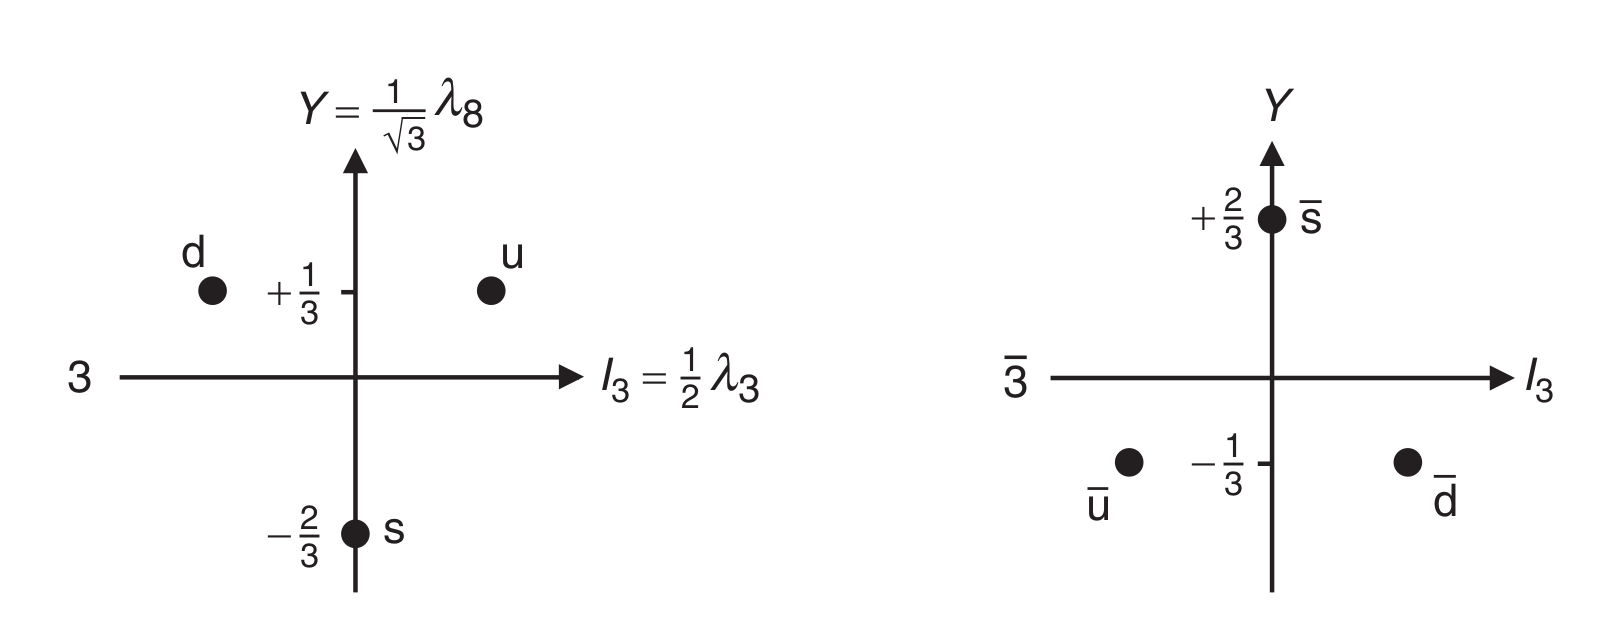
\includegraphics[width=0.6\textwidth]{Hypercharge.png}
\caption{\label{trailer}\emph{Incident wavepackets are uniformly distributed in impact parameter $\textbf{b}$.}}
\end{figure}  
\item Since we have used $\lambda_3$ and $\lambda_8$ to form what is know as the Cartan sub-algebra, we can take the remaining $\lambda_i$ and form raising and lowering operators. There will be three pairs, that which step respectively between the $d \leftrightarrow u, s\leftrightarrow u$ and $d\leftrightarrow s$:
\begin{align}
    \hat{T}_\pm &= \frac{1}{2} (\lambda_1 \pm i \lambda_2) \\
    \hat{V}_\pm &= \frac{1}{2} (\lambda_4 \pm i \lambda_5) \\
    \hat{U}_\pm &= \frac{1}{2} (\lambda_6 \pm i \lambda_7)
\end{align}
\end{itemize}
% subsection su3 (end)

\end{document}
